\title{Lecture 12: Probability in Board Game and Complex Number}

\frame{\titlepage}

%%%%%%%%%%%%%
\section{Advance}
\frame{\sectionpage}
%%%%%%%%%%%%%

\begin{frame}{Infinite Sum}
The formula for expected value still works if there are infinitely many outcomes. The following formula for geometric sum might be useful.
\begin{block}{Geometric sum}
If $-1 \leq r < 1$, then
\[ \sum_{n=0}^{\infty} r^n = 1 + r + r^2 + r^3 + \ldots = \frac{1}{1-r}\]
\end{block}
\end{frame}


\begin{frame}[t]
\begin{ex}
Suppose you flip a coin until you see a tail. What is the expected number of flips?
\end{ex}
\begin{sol}
Let $X$ be the number of coin flips until we get a tail. For $X = k$, there must be $k-1$ consecutive heads, and then 1 last tail. Since each flip is independent, the probability  is $\frac{1}{2^k}$. Hence,
\begin{eq*}
\red{E(X)} &=& \sum_{x = 1}^{\infty} x E(x) = \sum_{x=1}^{\infty} \frac{x}{2^x} =\frac{1}{2} + \frac{2}{4} + \frac{3}{8} + \frac{4}{16} + \ldots \\
\green{2E(X)} &=& 1 + \frac{2}{2} + \frac{3}{4} + \frac{4}{8} + \frac{5}{16} + \ldots \\
\green{2E(X)} -\red{E(X)} &=& 1 + \frac{1}{2} + \frac{1}{4} + \frac{1}{8} + \frac{1}{16} + \ldots \\
E(X) &=& 2
\end{eq*}
Thus, on average, we need to flip 2 times to see the first tail.
\end{sol}
\end{frame}

\begin{frame}
\frametitle{Recursive Formula}
It is possible that a formula of $E(X)$ contains the term $E(X)$ itself! This happens when there is a case when the experiment must be repeated.
\end{frame}


\begin{frame}[t]
\begin{ex}
Suppose you flip a coin until you see a tail. What is the expected number of flips?
\end{ex}
\begin{sol}
Let $X$ be the number of coin flips until we get a tail. 
\begin{itemize}
\item On a tail, the experiment ends and the number of flips is 1. 
\item On a head, the experiment is repeated, and the number of flips is $E(X) + 1$.
\end{itemize}
Thus, we have
\begin{eq*}
E(X) &=& (1) \frac{1}{2} + (E(X) + 1) \frac{1}{2} \\
E(X) &=& 1 + \frac{E(X)}{2} \\
E(X) &=& 2
\end{eq*}
This gives the same result as before.
\end{sol}
\end{frame}


\begin{frame}[t]
\begin{ex}
Suppose you roll a die. If the result less than 6, you get that much coins. If the result is 6, you must pay a penalty of 5 coins before rerolling again. What is the expected number of coins you would gain?
\end{ex}
\begin{sol}
Let $X$ be the amount of coins you gain. There is $\tfrac{1}{6}$ chance to roll a 1 and get 1 coin. There is $\tfrac{1}{6}$ chance to roll a 2 and get 2 coins, and so on. Finally, there is $\tfrac{1}{6}$ chance to roll a 6 and get $E(X) - 5$ coins. Thus, we have
\begin{eq*}
E(X) &=& (1) \frac{1}{6} + (2) \frac{1}{6} + (3) \frac{1}{6} + (4) \frac{1}{6} + (5) \frac{1}{6} + (E(X)-5) \frac{1}{6} \\
E(X) &=& \frac{10}{6} + \frac{E(X)}{6} \\
E(X) &=& 2
\end{eq*}
Thus, despite the heavy penalty, on average you still gain 2 coins!
\end{sol}
\end{frame}

%%%%%%%%%%%%%%%%%%
\section{Complex Dice Example}
\frame{\sectionpage}
%%%%%%%%%%%%%%%%%%

\begin{frame}{Risk}
\begin{itemize}
\item Attacker and Defender roll some dice. 
\item Sort dice on each side from highest to lowest.
\item Compare highest pair of dice. The smaller value loses 1 troop, when tied the attacker loses 1 troop.
\end{itemize}
\end{frame}


\begin{frame}
\addfig{0.8}{dice_risk.png}{Dice combat in Risk}
\end{frame}

\begin{frame}[t]
\begin{ex}
If attacker and defender each rolls a single die. Find the expected win for the attacker.
\end{ex}
\begin{sol}
Create a table listing all possible outcomes.
\begin{figure}[h!]
\centering
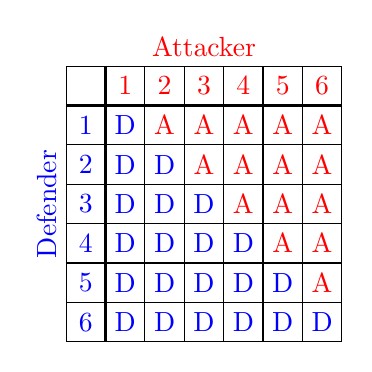
\begin{tikzpicture}[scale = 0.5, yscale = -1]
\draw (0,0) grid (7,7);
\draw[very thick] (1,0) -- (1,7) (0,1) -- (7,1);
\begin{scope}[xshift = 0.5cm, yshift = 0.5cm]
\node[red] at (3,-1) {Attacker};
\node[blue, rotate = 90] at (-1,3) {Defender};
\foreach \x in {1,2,3,4,5,6}
{
\node[red] at (\x, 0) {$\x$};
\node[blue] at (0, \x) {$\x$};
}
\foreach \attack in {1,2,3,4,5,6}
{
	\foreach \defend in {1,2,3,4,5,6}
	{
		\ifnum\attack > \defend
			\node[red] at (\attack, \defend) {A};
		\else
			\node[blue] at (\attack, \defend) {D};
		\fi 
	}
}
\end{scope}
\end{tikzpicture}
\end{figure}
We see that the attacker wins 15 out of 36 equally likely outcomes. Therefore, the expected win is $E(X) = \tfrac{15}{36} = \tfrac{5}{12}$ for each combat.
\end{sol}
\end{frame}

\begin{frame}[t]
\begin{ex}
If attacker rolls two dice and defender rolls one die. Find the expected loss for the attacker.
\end{ex}
\begin{sol}
First, let $X$ be the maximum of two dice for the attacker and determine $P(X)$ for each possible value. 
\begin{figure}[h!]
\centering
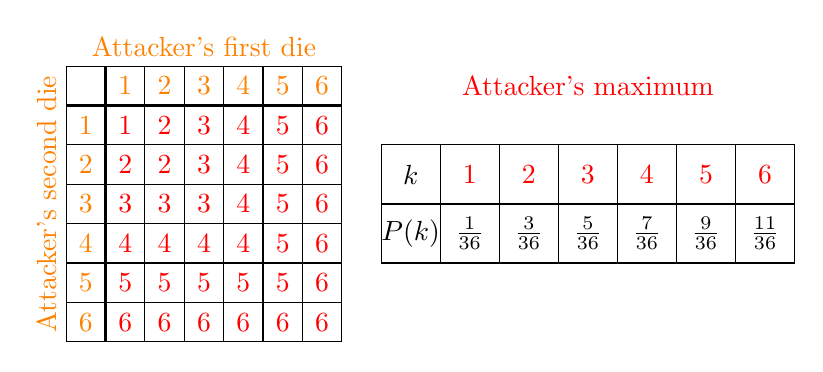
\begin{tikzpicture}[scale = 0.5, yscale = -1]
\draw (0,0) grid (7,7);
\draw[very thick] (1,0) -- (1,7) (0,1) -- (7,1);
\begin{scope}[xshift = 0.5cm, yshift = 0.5cm]
\node[orange] at (3,-1) {Attacker's first die};
\node[orange, rotate = 90] at (-1,3) {Attacker's second die};
\foreach \x in {1,2,3,4,5,6}
{
\node[orange] at (\x, 0) {$\x$};
\node[orange] at (0, \x) {$\x$};
}
\foreach \first in {1,2,3,4,5,6}
{
	\foreach \second in {1,2,3,4,5,6}
	{
		\ifnum\first > \second
			\node[red] at (\first, \second) {\first};
		\else
			\node[red] at (\first, \second) {\second};
		\fi 
	}
}
\end{scope}
% table on the right
\begin{scope}[xshift = 8cm, yshift = 2cm, scale = 1.5]
\draw (0,0) grid (7,2);
\node[red] at (3.5, -1) {Attacker's maximum};
\begin{scope}[xshift = 0.5cm, yshift = 0.5cm]
\node at (0,0) {$k$};
\node at (0,1) {$P(k)$};
\foreach \x /\p in {1/1,2/3,3/5,4/7,5/9,6/11}
{
\node[red] at (\x, 0) {$\x$};
\node at (\x,1) {$\frac{\p}{36}$};
}
\end{scope}
\end{scope}
\end{tikzpicture}
\label{}
\end{figure}
\end{sol}
\end{frame}

\begin{frame}[t]
\begin{sol} (Continued)
Then, we can apply these values to the previous table, but replacing a single win (A) with the actual probability from the second table.
\begin{figure}[h!]
\centering
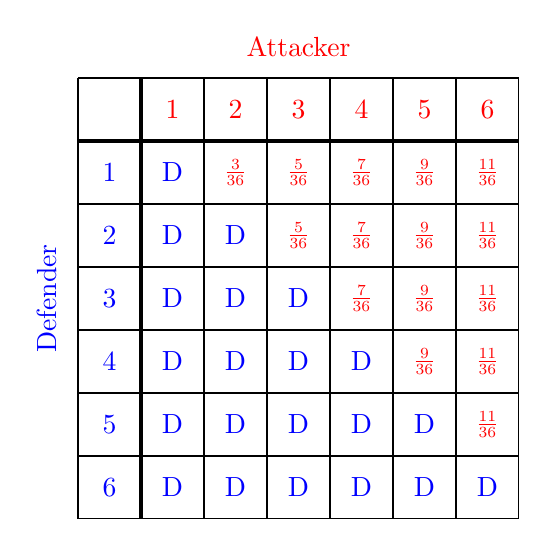
\begin{tikzpicture}[scale = 0.8, yscale = -1]
\draw (0,0) grid (7,7);
\draw[very thick] (1,0) -- (1,7) (0,1) -- (7,1);
\begin{scope}[xshift = 0.5cm, yshift = 0.5cm]
\node[red] at (3,-1) {Attacker};
\node[blue, rotate = 90] at (-1,3) {Defender};
\foreach \x in {1,2,3,4,5,6}
{
\node[red] at (\x, 0) {$\x$};
\node[blue] at (0, \x) {$\x$};
}
\foreach \attack / \p in {1/1,2/3,3/5,4/7,5/9,6/11}
{
	\foreach \defend in {1,2,3,4,5,6}
	{
		\ifnum\attack > \defend
			\node[red, scale = 0.8] at (\attack, \defend) {$\frac{\p}{36}$};
		\else
			\node[blue] at (\attack, \defend) {D};
		\fi 
	}
}
\end{scope}
\end{tikzpicture}
\end{figure}
\end{sol}
\end{frame}

\begin{frame}
\begin{sol} (Continued)
Here is how to interpret the table: in the first row when the defender rolls a 1, the attacker wins if they roll 2,3,4,5 or 6. Thus, the total in that case is $\frac{3}{36} + \frac{5}{36} + \frac{7}{36} + \frac{9}{36} + \frac{11}{36} = \frac{35}{36}$. 

\begin{figure}[h!]
\centering
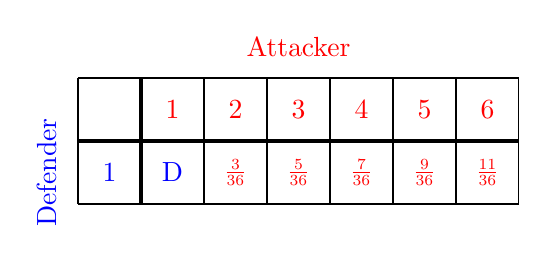
\begin{tikzpicture}[scale = 0.8, yscale = -1]
\draw (0,0) grid (7,2);
\draw[very thick] (1,0) -- (1,2) (0,1) -- (7,1);
\begin{scope}[xshift = 0.5cm, yshift = 0.5cm]
\node[red] at (3,-1) {Attacker};
\node[blue, rotate = 90] at (-1,1) {Defender};
\foreach \x in {1,2,3,4,5,6}
{
\node[red] at (\x, 0) {$\x$};
}
\node[blue] at (0,1) {1};
\foreach \attack / \p in {1/1,2/3,3/5,4/7,5/9,6/11}
{
	\ifnum\attack > 1
		\node[red, scale = 0.8] at (\attack, 1) {$\frac{\p}{36}$};
	\else
		\node[blue] at (\attack, 1) {D};
	\fi 
}
\end{scope}
\end{tikzpicture}
\end{figure}

Since the defender's values from 1-6 are equally likely, the expected number can be obtained by adding all red numbers. 
\[ E(X) = \frac{1}{6}\left(\frac{35}{36} + \frac{32}{36} + \frac{27}{36} + \frac{20}{36} + \frac{11}{36}\right) = \frac{125}{216}.\]
\end{sol}
\end{frame}

\begin{frame}{Yahtzee}
Roll 5 dice. You can keep any number of dice and reroll the rest. Then, you can keep any number of dice (either previously rerolled or not), and reroll the rest. Then the result is compared to a poker-hand-like table.
\end{frame}

\begin{frame}{}
\addfig{0.7}{dice_yahtzee}{Dice hand in Yahtzee}
\end{frame}

\begin{frame}[t]
\begin{ex}
Find the probability of getting a Yahtzee if you are allowed to reroll once (with any number of dice).
\end{ex}
\begin{sol}
\begin{itemize}
\item If our very first rolls give us a Yahtzee already, we win (yay!), with probability $\frac{6}{6^5}$.
\item If the first roll is four-of-a-kind, then we would reroll the last die. Now, the probability of getting four-of-a-kind is 
\[\frac{6 \times C(5,4) \times 5}{6^5} = \frac{150}{6^5}.\] 
We first consider which value to be the four-of-a-kind (6 possibilities), then which die to be the fifth unmatched die (5 chooses 4), and lastly which value to be on the fifth die (5 possibilities since it can't be the same with the rest).
\end{itemize}
\end{sol}
\end{frame}

\begin{frame}
\begin{sol} (Continued)
Therefore, the probability of getting a four-of-a-kind and then rerolling to get a Yahtzee is 
\[\frac{150}{6^5} \times \frac{1}{6} = \frac{25}{6^5}.\]
\begin{itemize}
\item If the first roll has three matching values, we apply a similar argument. The probability of getting such outcome is 
\[\frac{6 \times C(5,3) \times (5 \times 5)}{6^5} = \frac{1500}{6^5}.\] 
Then, the probability of rerolling two dice to match the first three is simply $\frac{1}{36}$. Thus, the probability is 
\[\frac{1500}{6^5} \times \frac{1}{36} = \frac{250}{6^6}.\]
\end{itemize}
\end{sol}
\end{frame}

%%%%%%%%%%%%%%%%%%
\section{Complex Number}
\frame{\sectionpage}
%%%%%%%%%%%%%%%%%%

% Section: Motivation
\begin{frame}{Intuition}
  \begin{itemize}
    \item Complex numbers appear in physics, engineering, and computer graphics.
    \item They let us solve equations that have no real solutions (e.g., $x^2+1=0$).
    \item Learning them builds algebra and geometric intuition.
  \end{itemize}
\end{frame}

\begin{frame}{Integers}
  \begin{itemize}
  \item First we have the set of natural numbers 
  \[\mathbb{N} =\{1,2,3,\ldots\}.\]
  \item Adding two natural numbers (says $3+9$) results in another natural number. This property is called closed: the set of natural numbers is closed under addition (and also multiplication).
  \item But subtracting one natural numbers from another does not always give you another natural number (says $5-8$).
  \item Fix: define negative numbers. Now we have the set of integers 
  \[\mathbb{Z} = \{\ldots, -2,-1,0,1,2\}.\]
  \end{itemize}
\end{frame}

\begin{frame}{Fractions}
  \begin{itemize}
  \item Great! Now adding, multiplying or subtracting two integers give you another integer.
  \item But now division doesn't work!
  \item Fix: define fractions. Now we have the set of rational numbers 
  \[\mathbb{Q} = \left\{\frac{a}{b} \Big| a,b \in \mathbb{Z}, b \neq 0 \right\}.\]
  \end{itemize}
\end{frame}

\begin{frame}{Fractions}
  \begin{itemize}
  \item Great! Now adding or subtracting two integers give you another integer.
  \item But the system is still flawed! There are numbers that can't be represented as a fraction of two integers, like the length of the hypotheuse of the right triangle with side lengths 1, or the circumference of a circle with radius 1.
  \begin{figure}[h!]
  \centering
  \begin{tikzpicture}[scale = 0.6]
  \begin{scope}[xshift =2cm]
  \draw (0,0) -- (2,0) node[pos=0.5, below] {$1$};
  \draw (2,0) -- (2,2) node[pos=0.5, right] {$1$};
  \draw (2,2) -- (0,0) node[pos=0.5, above left] {$?$};
  \end{scope}
  \draw[->] (0,1.1) arc[start angle = 0, end angle = 355, radius = 0.6] node[pos=0.5, left] {$?$};
  \end{tikzpicture}
  \end{figure}
  \item Fix: define ``decimal numbers''. Now we have the set of rational numbers 
\[\mathbb{R} = \left\{ x \, \Big| x \text{ can be written as an infinite decimal number.}\right\} \]
$\sqrt{2}$ and $\pi$ are real numbers because we can write $\sqrt{2} = 1.41421356\ldots$ and $\pi = 3.14159265\ldots$
  \end{itemize}
\end{frame}

\begin{frame}{Here comes the complex}
  \begin{itemize}
  \item Great! Now have all these fancy numbers!
  \item But the system is still flawed! Polynomials like
  \[x^2+1 = 0.\]
  do not have solutions as real numbers.
  \item Fix: assume they have solutions, which we defined as ``complex numbers''. Now we have the set of complex numbers $\mathbb{C} = \left\{ x \, | x  \text{ is a solution of a polynomial with real coefficients.}\right\}$.

  \end{itemize}
\end{frame}

\begin{frame}{The imaginary unit $i$}
\begin{thm}{}{}
Let $i$ be a root of the polynomial
\[x^2+1=0\]
\end{thm}
  \begin{itemize}
    \item We see that \(i^2 = -1.\)
    \item This seems strange because no real number squared gives $-1$.
    \item But we can treat $i$ as a new number that expands our number system.
  \end{itemize}
\end{frame}

\begin{frame}{Notation: Complex numbers}
  \begin{defn}{}{}
A \textbf{complex number} has the form 
\begin{equation}
z = a + bi,
\end{equation}
where $a$ and $b$ are real numbers.

\tcblower
$a$ is called the \textbf{real part} (\(\Re(z)=a\)), and $b$ is the \textbf{imaginary part} (\(\Im(z)=b\)).
\end{defn}
\end{frame}


\begin{frame}{Addition and subtraction}
\begin{thm}{}{}
Let $a+bi$ and $c+di$ be complex numbers. 
\begin{eq}
(a+bi) + (c+di) &=& (a + c) + (b + d)i \\
(a+bi) - (c+di) &=& (a - c) + (b - d)i
\end{eq}
\end{thm}
\end{frame}

\begin{frame}[t]
\begin{ex}
Compute the following additions.
\begin{tasks}(3)
\task $(3+2i) + (4-5i)$
\task $(4i) + (-2+3i)$
\task $(-1-i) + 5$
\end{tasks}
\end{ex}
\begin{sol}
\begin{tasks}(1)
\task $(3+2i) + (4-5i) = (3+4) + (2-5)i = 7-3i$
\task $(4i) + (-2+3i) = (0+(-2)) + (4+3)i = -2+7i$
\task $(-1-i) + 5 = (-1+5) + (-1+0)i = 4-i$
\end{tasks}
\end{sol}
\end{frame}

\begin{frame}[t]
\begin{ex}
Compute the following subtractions.
\begin{tasks}(3)
\task $(3+2i) - (4-5i)$
\task $(4i) - (-2+3i)$
\task $(-1-i) - 5$
\end{tasks}
\end{ex}
\begin{sol}
\begin{tasks}(1)
\task $(3+2i) - (4-5i) = (3-4) + (2-(-5))i = -1+7i$
\task $(4i) - (-2+3i) = (0-(-2)) + (4-3)i = 2+i$
\task $(-1-i) - 5 = (-1-5) + (-1-0)i = -6-i$
\end{tasks}
\end{sol}
\end{frame}

\begin{frame}{Multiplication}
Multiply like polynomials and use $i^2=-1$:
\begin{eq*}
(a+bi)(c+di) &=& ac + a(di) + (bi)c + (bi)(di) \\
&=& ac + (ad)i + (bc)i + bd(i^2) \\
&=& ac + (ad)i + (bc)i - bd \\
&=& (ac-bd) + (ad+bc)i
\end{eq*}
  \begin{thm}{}{}
    \begin{equation} 
    (a+bi)(c+di) = (ac - bd) + (ad+bc)i
    \end{equation}
  \end{thm}
Note: do not remember the formula! You should multiply complex numbers like polynomials.
\end{frame}


\begin{frame}[t]
\begin{ex}
Compute the following products.
\begin{tasks}(3)
\task $(3+2i)(4-5i)$
\task $(4i)(-2+3i)$
\task $(5)(-1-i)$
\end{tasks}
\end{ex}
\begin{sol}
\begin{eq*}
(3+2i)(4-5i) &=& (3)(4) + (3)(-5i) + (2i)(4) + (2i)(5i) \\
&=& 12 - 15i + 8i - 10 \\
&=& 22 - 7i \\
(4i)(-2+3i) &=& (4i)(-2) + (4i)(3i)\\
 &=& -8i - 12 \\
 &=& -12 - 8i \\
(5)(-1-i) &=& (5)(-1) + (5)(-i) \\
&=& -5-5i
\end{eq*}
\end{sol}
\end{frame}

\begin{frame}{Conjugate}
\begin{defn}{}{}
Complex conjugation is denoted with a bar and defined by
\begin{equation}
\overline{a+bi} = a-bi
\end{equation}
If $z=a+bi$, then its conjugate is $\overline{z} = a-bi$ and we read this as ``z-bar''  
\end{defn}

The complex conjugation has a useful property: if $z = a+bi$, then
\[z\overline{z} = (a+bi)(a-bi) = a^2 - (bi)^2 = a^2+b^2,\]
which has no imaginary part.
\end{frame}

\begin{frame}[t]
\begin{ex}
Find the complex conjugations of the following complex numbers.
\begin{tasks}(4)
\task $2+6i$
\task $-4-3i$
\task $8i$
\task $-7$
\end{tasks}
\end{ex}
\begin{sol}
\begin{tasks}(1)
\task $\overline{2+6i}=2-6i$
\task $\overline{-4-3i} = -4+3i$
\task $\overline{8i} = -8i$
\task $\overline{-7} = -7$
\end{tasks}
\end{sol}
\end{frame}

\begin{frame}{Division}
To divide, multiply numerator and denominator by the \textbf{conjugate} of the denominator.
\begin{thm}{}{}
\begin{equation}
\frac{a+bi}{c+di} = \frac{(a+bi)(c-di)}{(c+di)(c-di)} = \frac{(ac+bd) + (bc-ad)i}{c^2+d^2}
\end{equation}
\end{thm}
Again, do not remember this formula.
\end{frame}

%%%%%%%%%%%%%%%%
\section{Complex plane}
\frame{\sectionpage}
%%%%%%%%%%%%%%%%

\begin{frame}{Complex plane and rectangular form}
  \begin{columns}
    \column{0.4\textwidth}
      We can picture complex numbers on a plane: horizontal axis for the real part, vertical axis for the imaginary part.
      \begin{itemize}
        \item Point $(a,b)$ corresponds to $a+bi$.
        \item Example: $3-2i$ is the point $(3,-2)$.
      \end{itemize}
     We will call $a+bi$ a \text{rectangular form}, because $a$ and $b$ represent rectangle's width and height.
    \column{0.6\textwidth}
      \begin{center}
      \begin{tikzpicture}[scale=0.8]
        \draw[<->] (-3.5,0) -- (3.5,0) node[right]{Re};
        \draw[<->] (0,-3.5) -- (0,3.5) node[above]{Im};
        \foreach \x in {-3,-2,-1,1,2,3} \draw (\x,0.05)--(\x,-0.05) node[below=2pt]{\small\x};
        \foreach \y in {-3,-2,-1,1,2,3} \draw (0.05,\y)--(-0.05,\y) node[left=2pt]{\small\y};
        \filldraw[black] (2,1) circle (1.5pt) node[above right]{\small $2+i$};
        \filldraw[black] (3,-2) circle (1.5pt) node[below right]{\small $3-2i$};
      \end{tikzpicture}
      \end{center}
    \end{columns}
\end{frame}

\begin{frame}{Modulus (length) and argument (angle)}
It is very crucial to think of a complex number on the plane as a vector. Then, the addition and subtraction are defined in the same way.
\begin{eq*}
\text{vector addition: \quad } \bv{a,b} + \bv{c,d} &=& \bv{a+c, b+d} \\
\text{complex number addition: \quad} (a+bi) + (c+di) &=& (a+c) + (b+d)i
\end{eq*}

Then, we can define the following vector components.
\begin{defn}{}{}
  For $z=a+bi$:
  \begin{itemize}
    \item Modulus (distance from origin): $|z| = \sqrt{a^2 + b^2}$.
    \item Argument (angle with positive real axis): $\arg(z)=\theta$ where $\tan\theta = \frac{b}{a}$. (Ignore the quadrant for now....)
  \end{itemize}
  \end{defn}
\end{frame}

\begin{frame}{Drawing a vector and labeling}
  \begin{figure}[h!]
  \centering
    \begin{tikzpicture}[scale=1]
      \draw[->] (-1,0) -- (4,0) node[right]{Re};
      \draw[->] (0,-1) -- (0,3) node[above]{Im};
      \draw[thick,->] (0,0) -- (3,2) node[above, right]{$z=(3,2)$};
      \draw[dashed] (3,0) -- (3,2);
      \node at (1.8,0.2) {3};
      \node at (3.2,1) {2};
      \draw (0.8,0) arc (0:34:0.8) node[midway, left]{$\theta$};
    \end{tikzpicture}
  \end{figure}
\end{frame}

%%%%%%%%%%%%%%%%
\section{Polar Form}
\frame{\sectionpage}
%%%%%%%%%%%%%%%%

\begin{frame}{Euler's formula}
  \begin{thm}{}{}
  Recall that $e \approx 2.71828$. For any real number $\theta$, we have
    \begin{equation} 
    e^{i\theta} = \cos\theta + i\sin\theta
    \end{equation}
  \end{thm}
  The proof uses calculus knowledge (such as Taylor series of $e^x, \sin x$ and $\cos x$). Roughly, this implies that the operation $e^i$ represents a rotation.
  
\begin{remark}{}
There are two units for the angle $\theta$: degree and radian. In this lecture, we will only use degree, and so we will drop the degree notation $^\circ$.  
\end{remark}
\end{frame}

\begin{frame}{Polar form $(r,\theta)$}
\begin{defn}{}{}
A complex number $z =a+bi$ can also be epressed in polar form as 
\begin{eq}
z &=& r(\cos\theta + \sin\theta i) \\
&=& r e^{i\theta}
\end{eq} 
where $r=|z|$ is the modulus and $\theta=\arg(z)$ is the argument.
\tcblower
We have
\begin{eq}
a &=& r \cos \theta \\
b &=& r \sin \theta
\end{eq}
\end{defn}
\end{frame}

\begin{frame}{Drawing a vector and labeling}
  \begin{figure}[h!]
  \centering
    \begin{tikzpicture}[scale=1]
      \draw[->] (-1,0) -- (4,0) node[right]{Re};
      \draw[->] (0,-1) -- (0,3) node[above]{Im};
      \draw[thick,->] (0,0) -- (3,2) node[midway, above left] {$r$}; 
      \node at (3.2,2.5) {$z=a+bi = re^{i\theta}$};
      \draw[dashed] (3,0) -- (3,2);
      \node at (1.8,-0.2) {$a$};
      \node at (3.2,1) {$b$};
      \draw (0.8,0) arc (0:34:0.8) node[midway, below left]{$\theta$};
    \end{tikzpicture}
    \caption{Representing a complex number both in rectangular form $(a+bi)$ and polar form ($re^{i\theta}$)}
  \end{figure}
\end{frame}

\begin{frame}[t]
\begin{ex}
Change the following complex numbers in polar form to rectangular form.
\begin{tasks}(3)
\task $4e^{i \,30}$
\task $-5e^{i \,120}$
\task $\frac{1}{2} e^{i \,90}$
\end{tasks}
\end{ex}
\begin{sol}
\begin{tasks}
\task $4e^{i \,30} = 4(\cos (30) + \sin (30)i) = 4 \left( \frac{\sqrt{3}}{2} + i \frac{1}{2}\right) = 2 \sqrt{3} + 2i$
\task $-5e^{i \,120} = -5(\cos (120) + \sin (120)i) = -5 \left( \frac{-1}{2} + i \frac{\sqrt{3}}{2}\right) = \frac{5}{2} - \frac{5\sqrt{3}}{2}i$
\task $\frac{1}{2} e^{i \,90} = \frac{1}{2} (\cos (90) + \sin (90) i) = \frac{1}{2}(i) = \frac{i}{2}$
\end{tasks}
\end{sol}
\end{frame}

\begin{frame}{Multiplication in polar form}
The nice thing about the polar form is that multiplication, division, and powers become easier!
\begin{thm}{}{}
Let $z_1 = r_1 e^{i\theta_1}$ and $z_2 = r_2 e^{i\theta_2}$. Then
\begin{eq}
z_1 z_2 = r_1 r_2 e^{i(\theta_1 + \theta_2)}
\end{eq}
\end{thm}
Interpretation: to multiply two complex numbers, you can multiply lengths and add angles.
\end{frame}

\begin{frame}{Division in polar form}
\begin{thm}{}{}
Let $z_1 = r_1 e^{i\theta_1}$ and $z_2 = r_2 e^{i\theta_2}$. Then
\begin{eq}
\frac{z_1}{z_2} = \frac{r_1}{r_2} e^{i(\theta_1 - \theta_2)}
\end{eq}
\end{thm}
Interpretation: to divide two complex numbers, you can divide their lengths and subtract angles.
\end{frame}

\begin{frame}[t]
\begin{ex}
Find the multiplications in polar form.
\begin{tasks}(2)
\task $(3 e^{i \,90})(2 e^{i \,60})$
\task $(-e^{i \,180})\left( \frac{1}{2} e^{-i 90} \right)$
\end{tasks}
\end{ex}
\begin{sol}
\begin{eq*}
(3 e^{i \,90})(2 e^{i \,60}) &=& (3)(2) e^{i \,(90+60)} \\
&=& 6 e^{i \,(150)} \\
(-e^{i \,180})\left( \frac{1}{2} e^{-i 90} \right) &=& (-1)\left(\frac{1}{2}\right) e^{i \,(180+(-90)} \\
&=& -\frac{1}{2}e^{i \,90}
\end{eq*}
\end{sol}
\end{frame}

\begin{frame}{Powers: De Moivre's theorem}
Notice that if we multiply repeatedly, we have
\begin{eq*}
(r e^{i\theta})^2 &=& (r e^{i\theta}) (re^{i\theta}) = r^2 e^{i \,(2\theta)} \\
(r e^{i\theta})^3 &=& (r e^{i \,\theta}) (r e^{i\theta})^2 = r^3 e^{i \,(3\theta)}.
\end{eq*}
Indeed, this observation is true for any positive power!
\begin{thm}{De Moivre}{}
Let $r$ and $\theta$ be real numbers and $n$ be a positive real number. Then, we have
\begin{equation}
(r e^{i\theta})^n = r^n e^{in\theta}
\end{equation}
\end{thm}
\end{frame}

\begin{frame}[t]
\begin{ex}
Compute the following powers.
\begin{tasks}(2)
\task $(2e^{i \,45})^4$
\task $\left(\frac{1}{3} e^{i \,30} \right)^3$
\end{tasks}
\end{ex}
\begin{sol}
\begin{tasks}(1)
\task $(2e^{i \,45})^4 = 2^4 e^{i \,(4 \times 45)} = 16e^{i \,180}$
\task $\left(\frac{1}{3} e^{i \,30} \right)^3 = \left(\frac{1}{3}\right)^3 e^{i \,(3 \times 30)} = \frac{1}{27} e^{i \,90}$
\end{tasks}
\end{sol}
\end{frame}


\begin{frame}[t]
\begin{ex}
Find a complex number $z$ such that $z^3 = 125 e^{i \, 60}$.
\end{ex}
\begin{sol}
If we write $z = re^{i\theta}$, then $z^3 = r^3 e^{i (3\theta)}$. We can simply compare
\[r^3 e^{i \,(3\theta)} = 125 e^{i \, 60}\]
so that we have $r^3=125$ and $3\theta = 60$. These give use $r=5$ and $\theta = 20$, and thus
\[z = 5 e^{i \, 20}\]
is a complex number such that $z^3 = 125 e^{i \, 60}$.
\end{sol}
\end{frame}

\begin{frame}{An n-th root}
In the previous example, we have
\[ z^3 = 125 e^{i \, 60} \]
and then we can write
\[z = (125 e^{i \, 60}) ^{\frac{1}{3}}.\]

In particular, we have the following definition
\begin{defn}{}{}
Let $z$ and $w$ be complex numbers and $n$ be a positive integer such that $z^n = w$. Then we have
\[z = w^{\frac{1}{n}}\]
and call $z$ an n-th root of $w$.
\end{defn}
\end{frame}

%%%%%%%%%%%%%%%%
\section[Roots]{Roots of Complex Numbers}
\frame{\sectionpage}
%%%%%%%%%%%%%%%%

\begin{frame}{Roots of unity}
Consider the polynomial
\[x^n = 1\]
where $n$ is a natural number. We know that
\begin{eq*}
x^2=1 &\rightarrow& x = -1,1\\
x^3 = 1 & \rightarrow& x = 1 \\
x^4 = 1 & \rightarrow& x = -1, 1
\end{eq*}
and so on. Note that $x^3=1$ has one real root $x=1$, but the degree of 3 suggests there should be 3 roots in total. Using complex numbers, we can find the other two roots.
\end{frame}

\begin{frame}{}
We rewrite the equation as 
\[x^3 = 1\]
If $x = re^{i\theta}$, then
\[x^3= r^3e^{i(3\theta)}\]

We see that $r=1$ since the modulus (or length) of the right-handed side is 1. However, $\theta$ requires attention because note that
\[1 = e^{i \, 0}\]
and setting $3\theta = 0$ gives us $\theta = 0$as one solution. But actually, using trigonometry we have
\[1 = e^{i \, (360 k)} \]
where $k$ is an integer. This means that we can rotate the complex number $360$ degree and get the same number as the origin. Thus, the correct equation would be
\[3 \theta = 360 k \]
\end{frame}

\begin{frame}{}
Finally, we have
\begin{eq*}
(k=0) \quad 3\theta = 0 &\rightarrow& \theta = 0 \\
(k=1) \quad 3\theta = 360 & \rightarrow& \theta = 120 \\
(k=2) \quad 3\theta = 720 & \rightarrow& \theta = 240 \\
(k=3) \quad 3\theta = 1080 & \rightarrow& \theta = 360
\end{eq*}
But $\theta = 0$ and $\theta = 360$ are the same angle and thus yields the same solution. Thus, the roots of the polynomial $x^3=1$ are
\[x = 1, e^{i \,120}, e^{i \, 240},\]
or, in the form $z=a+bi$, we have
We can repeat the same argument for any power $x^n$
\end{frame}

\begin{frame}{Roots of Unity}
\begin{thm}{}{}
The roots of $x^n=1$ where $n$ is a natural number are
\begin{equation}
x = e^{i \,\frac{360 k}{n}}, k=0,1,2,\ldots,n-1
\end{equation}
These are called ``roots of unity'' of degree $n$. Geometrically, these are unit vectors equally spaced around the origin.
\end{thm}
\end{frame}

\begin{frame}[t]
\begin{figure}[h!]
\centering
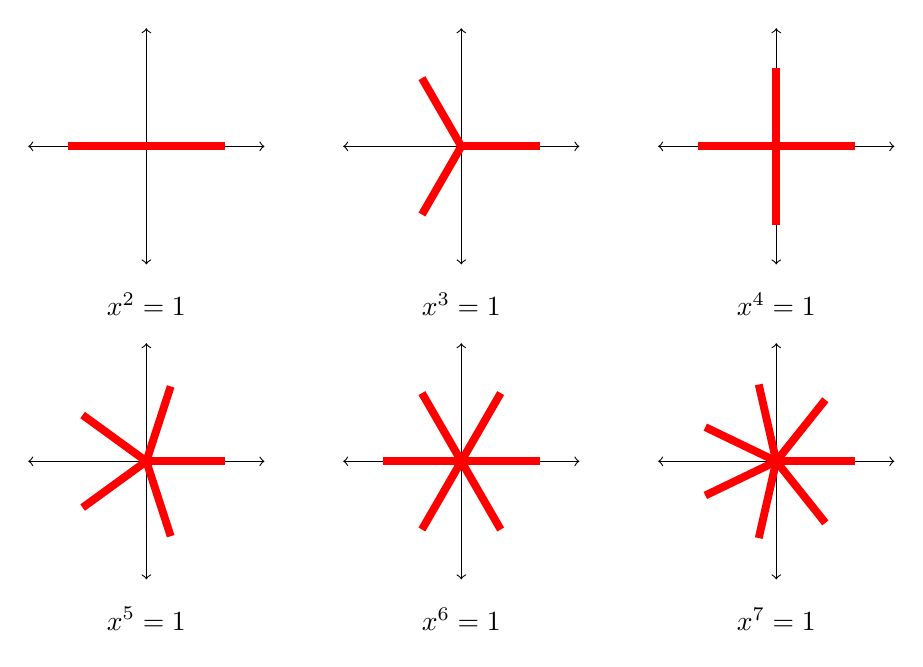
\begin{tikzpicture}
\foreach \n / \x / \y in {2/1/1,3/2/1,4/3/1,5/1/2,6/2/2,7/3/2} {
	\begin{scope}[xshift = {4*\x cm}, yshift={-4*\y cm}] 
		\draw[<->] (-1.5,0)--(1.5,0);
		\draw[<->] (0,-1.5)--(0,1.5);
		\foreach \k in {0,1,...,\n} {
			\draw[line width = 0.1cm, red] (0,0) -- ({\k*360/\n}:1cm);
		}
		\node at (0, -2) {$x^{\n} = 1$};
	\end{scope}
}
\end{tikzpicture}
\caption{}
\label{}
\end{figure}
\end{frame}

\begin{frame}[t]
\begin{ex}
Find the roots of unity of degree 4.
\end{ex}
\begin{sol}
Applying the theorem, the roots are
\[x = e^{i \,\frac{360k}{4}}, k=0,1,2,3\]
These are $e^{i0}, e^{i \, 90}, e^{i \, 180}, e^{i \, 270}$, which can also be expressed as $1, i, -1, -i$.
\end{sol}
\end{frame}


\begin{frame}{N-th roots}
For any complex number $z = re^{i\theta}$, recall that we can find an n-root using De Moivre's rule.
\[ z^{\frac{1}{n}} = r^{\frac{1}{n}} e^{i \left(\frac{\theta}{n}\right)}\]
Now, we can indeed find \text{all} roots using roots of unity.
\begin{thm}{}{}
Let $z=re^{i\theta}$ be a complex number and $n$ be a natural number. The n-th roots of $z$ are
\begin{equation}
z_k = r^{\frac{1}{n}} e^{i \,\frac{\theta + 360k}{n}}, k=0,1,2,\ldots,n-1
\end{equation}
We have $z_k^n = z$.
\end{thm}
\end{frame}

\begin{frame}[t]
\begin{ex}
Find all cube roots of 8.
\end{ex}
\begin{sol}
Write $8 = 8 e^{i \,0}$. Cube roots are:
\[ 8^{1/3} e^{i \, \frac{0 + 360k}{3}} = 2 e^{i \, (120 k)},\quad k=0,1,2. \]
These are: $2,\; 2e^{i \, 120}$ and $\; 2e^{i \, 240}.$
\end{sol}
\end{frame}

\begin{frame}[t]
\begin{ex}
Find all fourth roots of -81.
\end{ex}
\begin{sol}
Write $-81 = 81 e^{i \,180}$. Cube roots are:
\[ 81^{1/4} e^{i \, \frac{180 + 360k}{4}} = 3 e^{i \, (45 + 90k)},\quad k=0,1,2,3. \]
These are: $3 e^{i \, 45}, 3e^{i \, 135}, 3e^{i\, 225}$ and $3e^{i \, 315}.$
\end{sol}
\end{frame}